\chapter{Introduction}

Memory could be defined as the biological storage for the information acquired from past experience with the environment. Human memory has been scientifically studied for at least 100 years~\cite{baddeley1997human} and today we know that there are many types of memory, all cooperating in the process of memorization so that they could be used to govern subsequent behavior of each individual. Memory is not a single unitary system such as the heart, but a collections of systems where one system is responsible for the encoding of new information while another system helps with its storage over a long period of time. The systems responsible for retention of information in the human brain are also very closely related to \textit{learning} and \textit{forgetting}, both of which in turn depend to some extent on memory. That is true because our memory provides the means and structure to link new knowledge faster by association and inference. Hence, human memory is a \textit{complex system} and the whole underlying process is still broadly studied by researchers who try to understand the complex cognitive processes by exploring the different memory systems of animals (e.g. rats) or patients who suffer amnesia as a consequence of brain damage~\cite{mcclelland1995there}.

The exploration of human memory and learning has applications particularly in education, where our goal is to increase the amount of material students learn in one study session. Before the invention of computers and the growth of the Internet, the ways to test and evaluate new methods of educating students involved classrooms with usually only a limited number of participants. In the last 20 years, students and educational institutions started to use and develop new e-learning systems as a complimentary tool for education. \textit{Adaptive educational systems} (sometimes referred as adaptive practice systems) are systems that provide online environment for practicing different domains of educational content adaptively.

In adaptive educational systems, our effort is to create sufficiently accurate representation of students in order to make the system personalized, increase students' motivation and the speed of learning. A part of all adaptive systems are mathematical models which are constructed in order to model learning of individual students and adapt the system to students' abilities, behavior and knowledge of the subject. These models and their evaluation is very often based on \textit{machine learning} techniques and is closely related to statistics. The ability to model the adaptive behavior also requires research connected to cognitive psychology.

One example of a free web-based adaptive educational system is the project called Outline Maps\footnote{Available at \href{http://outlinemaps.org}{\texttt{outlinemaps.org}}} developed at the Faculty of Informatics at Masaryk University. This project helps students practice all kinds of geography facts~\cite{Papousek2014}, including world countries, cities, rivers, lakes, mountains, islands, Czech regions, and many others. The practice procedure of geography in the system involves rehearsal of contextual information about a place on a map, i.e. the location, shape or neighbors of a country. The test of students' knowledge is done by presenting questions requiring the identification of correct association between a name of a place and its position on an outline map (see Figure~\ref{fig:slepemapy}).

\begin{figure}[htbp]
  \centering
  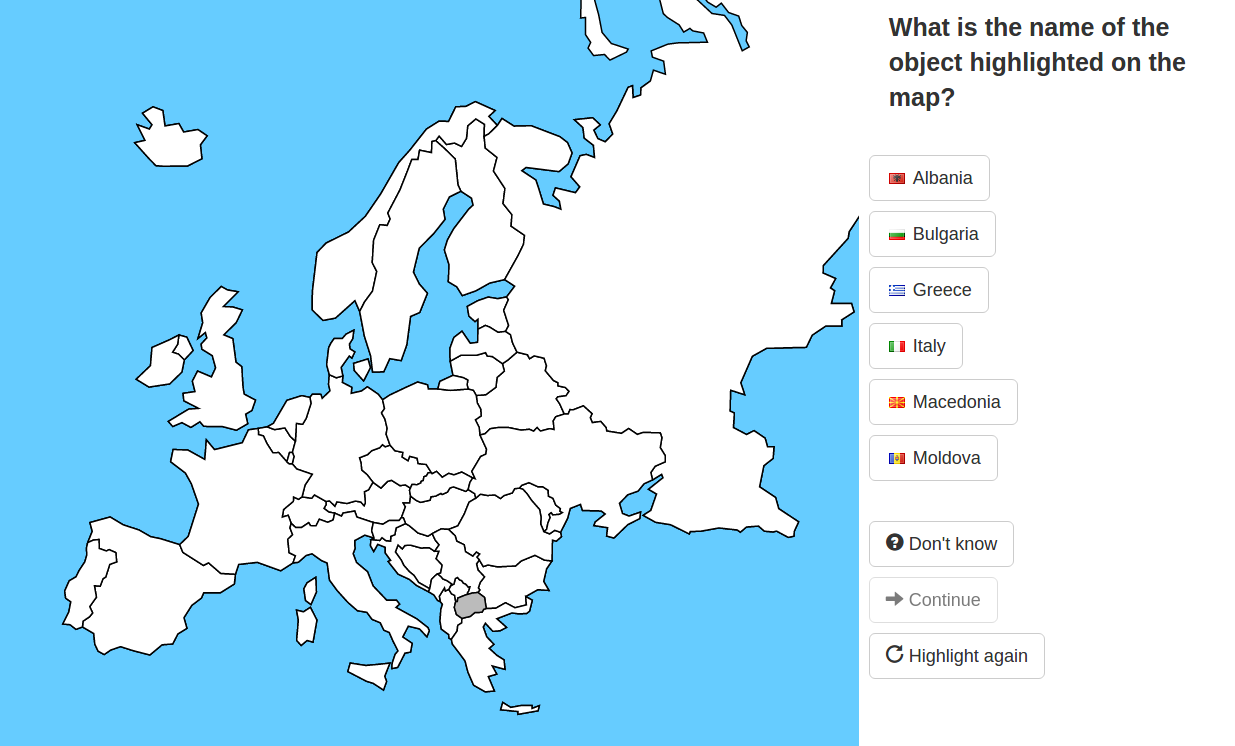
\includegraphics[width=\textwidth]{img/slepemapy}
  \caption{The screenshot corresponds to a multiple-choice question (with 5 distractors) requiring the student to identify the name of the highlighted country on an outline map of Europe.}
  \label{fig:slepemapy}
\end{figure}

Since the system is adaptive, it examines knowledge and skills of students adaptively based on previous answers---by the selection of optimal repeat frequency, the type of question, its difficulty etc. In this context, the practice of geography is somewhat different from ordinary memorization of vocabulary pairs as there are bigger variations in the prior knowledge of individual students.

\section{Objectives}

The first objective of the thesis is to study the related research to modeling human memory and forgetting mainly in the context of adaptive educational systems. The first objective also involves the study of the relevant machine learning models and the determination of which one is the best candidate considering all its aspects.

Our primary objective is to design, evaluate and analyze the models suitable for adaptive practice systems while accounting for key aspects of human memory and forgetting. The findings should provide insights into how modeling the effect of forgetting improves model's performance. We are particularly interested with student modeling for application in the adaptive system Outline Maps.

\section{Outline}

The second chapter covers the background of our thesis, we summarize the most relevant attributes of human memory and forgetting that are related to our research, we also describe characteristics of adaptive educational systems as well as mathematical models used in student modeling. In the third chapter, we propose models and their modifications that focus on \textit{timing information} (e.g. the ages of student's past trials and response times), we also describe the methods commonly used in machine learning for parameter estimation and metrics for the quantification of model's performance. The fourth chapter includes evaluation of the proposed models and further analysis of their parameters. Finally, the last chapter concludes the results of our experiments and outlines suggestions for possible future research.
